\chapter{State of the art system identification analysis}
\label{identification_methods}

\emph{In this chapter, first an overview is given about the different steps that one has to consider in non-linear system identification. Secondly, different approaches are explained and compared. As a conclusion of the comparison, the selected approach is further discussed which leads to the introduction of Artificial Neural Networks(ANNs). Afterwards, the system identification and validation is carried out using the available data from the EPANET framework.}

\section{Tasks in non-linear system identification}
\label{tasks_nonlinear_sys_identification}

Modelling and identification of non-linear systems is a challenging task because non-linear processes do not share properties such as the superposition in linear systems. In this sense, non-linear systems are unique and the methods for describing structurally different systems are complex. However, as for any identification method, the goal is to find a model which is capable to represent the behaviour of a process as closely as possible. The quality of the model is typically measured in terms of the error between the output of the process and the model. In \figref{fig:nonlin_block} an illustration is shown for a system identification arrangement 
\vspace{-3mm}
 %Non-lin system identification 
\begin{figure}[H]
\centering
%
\includegraphics[width=0.35\textwidth]{report/pictures/missingfigure}
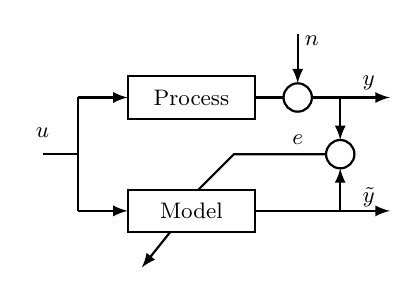
\begin{tikzpicture}[scale=0.9,transform shape]

\draw [thick] (-3,3) rectangle (-1.2,2.4);
\node at (-2.1,2.7) {\small Process};
\node at (-2.1,1.1) {\small Model};
\node at (-4.2,2.2) {\small $u$};
\node at (-0.4,3.5) {\small $n$};
\node at (-0.6,2.1) {\small $e$};
\node at (0.4,1.3) {\small $\tilde{y}$};
\node at (0.4,2.9) {\small $y$};


\draw [thick] (-3,1.4) rectangle (-1.2,0.8);
\draw [thick] (-0.6,2.7) ellipse (0.2 and 0.2);
\draw [thick] (0,1.9) ellipse (0.2 and 0.2);
\draw [thick][-latex](-0.4,2.7) -- (0.7,2.7);
\draw [thick][-latex](0,2.7) -- (0,2.1);
\draw [thick][-latex](-1.2,1.1) -- (0,1.1) -- (0,1.7);
\draw [thick](-0.2,1.9) -- (-1.5,1.9) -- (-2,1.4);
\draw [thick](-1.2,2.7) -- (-0.8,2.7);
\draw  [thick][-latex](-2.4,0.8) -- (-2.8,0.3);
\draw  [thick][-latex](0.0,1.1) -- (0.7,1.1);
\draw [thick][-latex](-3.7,2.7) -- (-3,2.7);
\draw [thick][-latex](-3.7,1.1) -- (-3,1.1);
\draw [thick](-3.7,2.7) -- (-3.7,1.1);
\draw [thick](-4.2,1.9) -- (-3.7,1.9);
\draw  [thick][-latex](-0.6,3.6) -- (-0.6,2.9);
\end{tikzpicture} 
\vspace{-3mm}
\caption{Block diagram of system identification \cite{nelles2013nonlinear}.}
\label{fig:nonlin_block}
\end{figure}

\vspace{-4mm}

The process and model are fed with the same input signals, and their outputs are compared. This comparison gives an error signal $e$, which can be utilized for adapting the model. It should be noted, that in most cases the measurements on the output are disturbed by noise $n$. In order to carry out a succesful system identification, some major steps need to be performed, either by user interaction or using algorithms which can automatize these steps. \figref{fig:identification_loop} shows the system identification loop with the major steps

 %system identification algorithm 
\begin{figure}[H]
\centering
%
\includegraphics[width=0.35\textwidth]{report/pictures/missingfigure}
\usetikzlibrary{arrows}
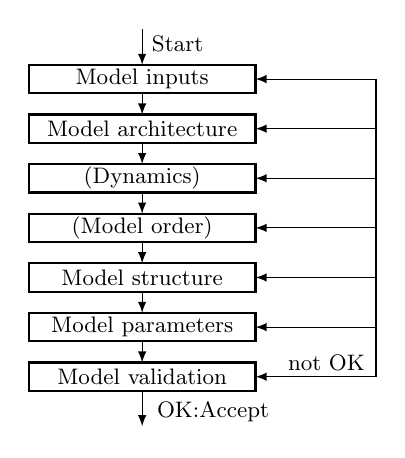
\begin{tikzpicture}[scale=0.9,transform shape]

\draw [thick] (-9.7,6.2) rectangle (-6.5,5.8);
\draw [thick] (-9.7,5.5) rectangle (-6.5,5.1);
\node at (-8.1,6) {\small Model inputs};

\node at (-8.1,5.3) {\small Model architecture};
\node at (-8.1,4.6) {\small (Dynamics)};
\node at (-8.1,3.9) {\small (Model order)};
\node at (-8.1,3.2) {\small Model structure};
\node at (-8.1,2.5) {\small Model parameters};
\node at (-8.1,1.8) {\small Model validation};
\node at (-7.6,6.5) {\small Start};
\node at (-7.1,1.3) {\small OK:Accept};
\node at (-5.5,2) {\small not OK};

\draw [thick][-latex] (-9.7,4.1) rectangle (-6.5,3.7);
\draw [thick][-latex] (-9.7,4.4) rectangle (-6.5,4.8);
\draw [thick][-latex] (-9.7,3.4) rectangle (-6.5,3);
\draw [thick][-latex] (-9.7,2.7) rectangle (-6.5,2.3);
\draw [thick][-latex] (-9.7,2) rectangle (-6.5,1.6);
\draw [-latex](-8.1,5.8) -- (-8.1,5.5);
\draw [-latex](-8.1,5.1) -- (-8.1,4.8);
\draw [-latex](-8.1,4.4) -- (-8.1,4.1);
\draw [-latex](-8.1,3.7) -- (-8.1,3.4);
\draw [-latex](-8.1,3) -- (-8.1,2.7);
\draw [-latex](-8.1,2.3) -- (-8.1,2);
\draw [-latex](-8.1,1.6) -- (-8.1,1.1);
\draw [-latex](-8.1,6.7) -- (-8.1,6.2);
\draw [thick](-4.8,6) -- (-4.8,1.8);
\draw [-latex](-4.8,6) -- (-6.5,6);
\draw [-latex](-4.8,5.3) -- (-6.5,5.3);
\draw [-latex](-4.8,4.6) -- (-6.5,4.6);
\draw [-latex](-4.8,3.9) -- (-6.5,3.9);
\draw [-latex](-4.8,3.2) -- (-6.5,3.2);
\draw [-latex](-4.8,2.5) -- (-6.5,2.5);
\draw [-latex](-4.8,1.8) -- (-6.5,1.8);
\end{tikzpicture} 
\caption{System identification loop \cite{nelles2013nonlinear}.}
\label{fig:identification_loop}
\end{figure}

\vspace{-3mm}

Some of these steps in \figref{fig:identification_loop} are discussed in the further sections. Furthermore, in the following, the term Training Set(TS) is used to characterize the measurement data that is utilized to carry out the presented identification steps. A TS consists of $N$ input-output pairs such that

\begin{equation}
  \label{training set}
  \mathcal{D} = \{u_i , y_i\}_{i = 1,2, ..., N}.
\end{equation}

\subsection{Choice of the model inputs}
\label{choice_of_the_model_inputs}

The first step in the identification is typically realized by a trial-and-error approach with the help of prior knowledge. In physical systems such as a WSS, the influence of the different variables is quite clear and the inputs can be chosen by the model equations which were presented in \secref{multi_inlet_multi_WT_model}. It should be noted that in more complex systems, where the number of inputs are high and their influence is not so well defined, some data-driven input selection might be very helpful. In this case, using all inputs can lead to extremely high-dimensional approximation problems, which implies the need for a huge number of parameters and increases the training time. Techniques for input data selection such as Principal Component Analysis(PCA) can be utilized in order to decide the relevance of certain inputs on the system. The main drawback of such techniques is that the relevance of an input is dependant only on the input data distribution, therefore sometimes highly relevant inputs are removed \cite{nelles2013nonlinear}.  Other techniques, such as correlation analysis for linear systems or genetic algorithms for non-linear systems can be also utilized, however it is not discussed further in the report, as in our case all inputs are relevant. 

Furthermore, the choice of the input signal requires some prior knowledge about the operation of the system and the purpose of the model. For black box modelling, the measurement data is the most important source of information. The behaviour of the real world system that is not represented in the TS, cannot be described in the model, unless prior knowledge is explicitly incorporated. Therefore, the TS needs to be as representative as possible in order to incorporate the desired operation of the real world system. 
\vspace{-3mm}
\subsection{Choice of the model structure}
\label{choice_of_the_model_architecture}

The choice of the model architecture among many factors, depends on the type of the problem, the intended use, the insight into the real system behaviour, the complexity and the available data. The type of the problem can be for instance the approximation of a static system, or identification of the dynamics. In our case, both of them are considered. The intended use for the model architecture can differ whether the model is to be used for simulation, control, fault detection, etc. Considering the insight, the complexity and the available data, three different modelling approaches can be distinguished\cite{nelles2013nonlinear}. These approaches are compared in \tabref{comparisontable_sysid}. 

\vspace{-3mm}

\begin{center}
    \begin{tabular}{ | >{\centering\arraybackslash}m{1.8cm} | >{\centering\arraybackslash}m{3.6cm} | >{\centering\arraybackslash}m{3.6cm} | >{\centering\arraybackslash}m{3.6cm} |}
    \hline
    \multirow{1}{*}
     & \textbf{White box} & \textbf{Gray box} & \textbf{Black box} \\ 
     \hline
     \multirow{1}{*}
    \textbf{Information sources} & First principles and insights. &  Some insights and some data. & Data and experiments.\\ 
    \hline
      \multirow{1}{*}
    \textbf{Features} & Good understanding, high reliability and scalability. & $\longleftrightarrow$  & Short development time and insight is not required.\\ 
    \hline
      \multirow{1}{*}
    \textbf{Drawbacks} & Well described process is required. & $\longleftrightarrow$ & Not scalable and the accuracy is restricted by the available data.\\ 
    \hline
          \multirow{1}{*}
    \textbf{Application} & Planning, simulation and design for simple processes. & $\longleftrightarrow$ & Only for existing, rather complex processes.\\ 
    \hline
    \end{tabular}
    \captionof{table}{Comparison of system identification modelling approaches\cite{nelles2013nonlinear}.}
    \label{comparisontable_sysid}
\end{center}

As shown in \tabref{comparisontable_sysid}, White box models are completely derived by first principles, i.e., by physical laws. The parameters and equations, describing the whole network can be determined by theoretical modelling, as it was done for our system in \chapref{system_modelling}. Black box models however, are based on measurement data, which means that the model describing the system is developed by the characteristics of the data. In order to carry out a successful Black box modelling, very little insight or prior knowledge is required, however it is important to have a well-describing TS. The combination or compromise between Black and White box models is called Gray box modelling. In this case, the knowledge from first principles and the information contained in the measurement data are both utilized. The blank fields in \tabref{comparisontable_sysid} for Grey box models are left blank because the properties of such models lie between White and Black box modelling. Typically, when Grey box modelling is considered, the main goal is to overcome some of the most restrictive factors of the White and Black box approaches for the specific application. For example, some prior knowledge might be incorporated into a Black box model in order to ensure reasonable behaviour\cite{nelles2013nonlinear}. 

Often the structure may be determined by first principles but the model parameters may be estimated from data. It is important to note, that the WSS model presented in \chapref{system_modelling} has been derived by first principles, however due to complexity of the system and the available data, the identification will be carried out by Black box identification and approximation methods. 

\subsection{Model validation}
\label{model_validation}

The easiest type of validation is to check the quality of the model on the TS. If this does not give satisfactory results, the model is not accepted. In this case, it can be either concluded that information is missing from the input or the model is not flexible enough to describe the corresponding input-output relations. In case if the performance achieved on the TS is acceptable, it is desirable to test the model on a new data set, especially if noise is present in the system. It should be noted however, that this new testing data should excite the system in the same operating regions, as the model was trained on. Otherwise, the model fails the validation. 
